%\documentclass[twoside]{elsart}
%\documentclass[11pt,titlepage]{article}
\documentclass[12pt]{article}
\usepackage{graphicx}
\usepackage{sidecap}
\usepackage{caption2}
\usepackage{subfigure}

% Use the option doublespacing or reviewcopy to obtain double line spacing
% \documentclass[doublespacing]{elsart}

% if you use PostScript figures in your article
% use the graphics package for simple commands
% \usepackage{graphics}
% or use the graphicx package for more complicated commands
% \usepackage{graphicx}
% or use the epsfig package if you prefer to use the old commands
%\usepackage{epsfig}

% The amssymb package provides various useful mathematical symbols
\usepackage{amssymb}

%\usepackage{rotating}  % needed for shower
%\usepackage{psfrag,graphicx} % needed for StartDetector
%\usepackage{subfigure}

%\newlength{\marginswitch}
%\setlength{\marginswitch}{\evensidemargin}
%\setlength{\evensidemargin}{\oddsidemargin}
%\setlength{\oddsidemargin}{\marginswitch}

\setlength{\topmargin}{0pt}
\setlength{\evensidemargin}{2pt}
\setlength{\oddsidemargin}{2pt}
\setlength{\marginparwidth}{0pt}
\setlength{\marginparsep}{0pt}
\setlength{\textheight}{595pt}
\setlength{\textwidth}{480pt}
\newlength{\mylinewidth}
\setlength{\mylinewidth}{\linewidth}
\setlength{\leftmargin}{2pt}
\setlength{\rightmargin}{2pt}

\title{Definitions of TPC related track properties} 
\author{} 

\begin{document}
\begin{minipage}[20]{400pt}
\pagestyle{empty}
\begin{center}
ALICE Internal Note \\ ALICE-INT-2011-XXX
%\put(125,60){\includegraphics[width=0.2\textwidth]{../godlo.eps}}
\maketitle
\begin{abstract}
This document is supposed to help users in the analysis of ALICE TPC data.
\end{abstract}
\end{center}
\end{minipage}

\setcounter{page}{1}

\section{Definitions}

\subsection{Clusters}
	
	\begin{description}
	
	\item[TPC cluster.] A charged particle traversing the TPC induces a signal on a given pad-row. If the charge in a search window of 5 pads in wire direction and 5 bins in time direction exceeds a certain threshold and fulfills all necessary quality criteria, it is called a cluster. Therefore the maximum number of clusters per track is 159 which corresponds to the number of pad rows in a given TPC sector. Curling track parts are reconstructed as separate tracks.
	
\medskip
	{\it Number of TPC clusters:} $n_{cl}$ / {\tt AliESDtrack::GetTPCNcls() } 
\medskip
	
	The number of clusters assigned to a track is related to the track length in the sense that low $p_{t}$-tracks which do not reach the outer wall of the TPC have less clusters assigned. However, the relation is not straightforward, because the pad length in the TPC is increasing with radial distance to the center.
	
	
\begin{figure}[htbp]
\begin{center}
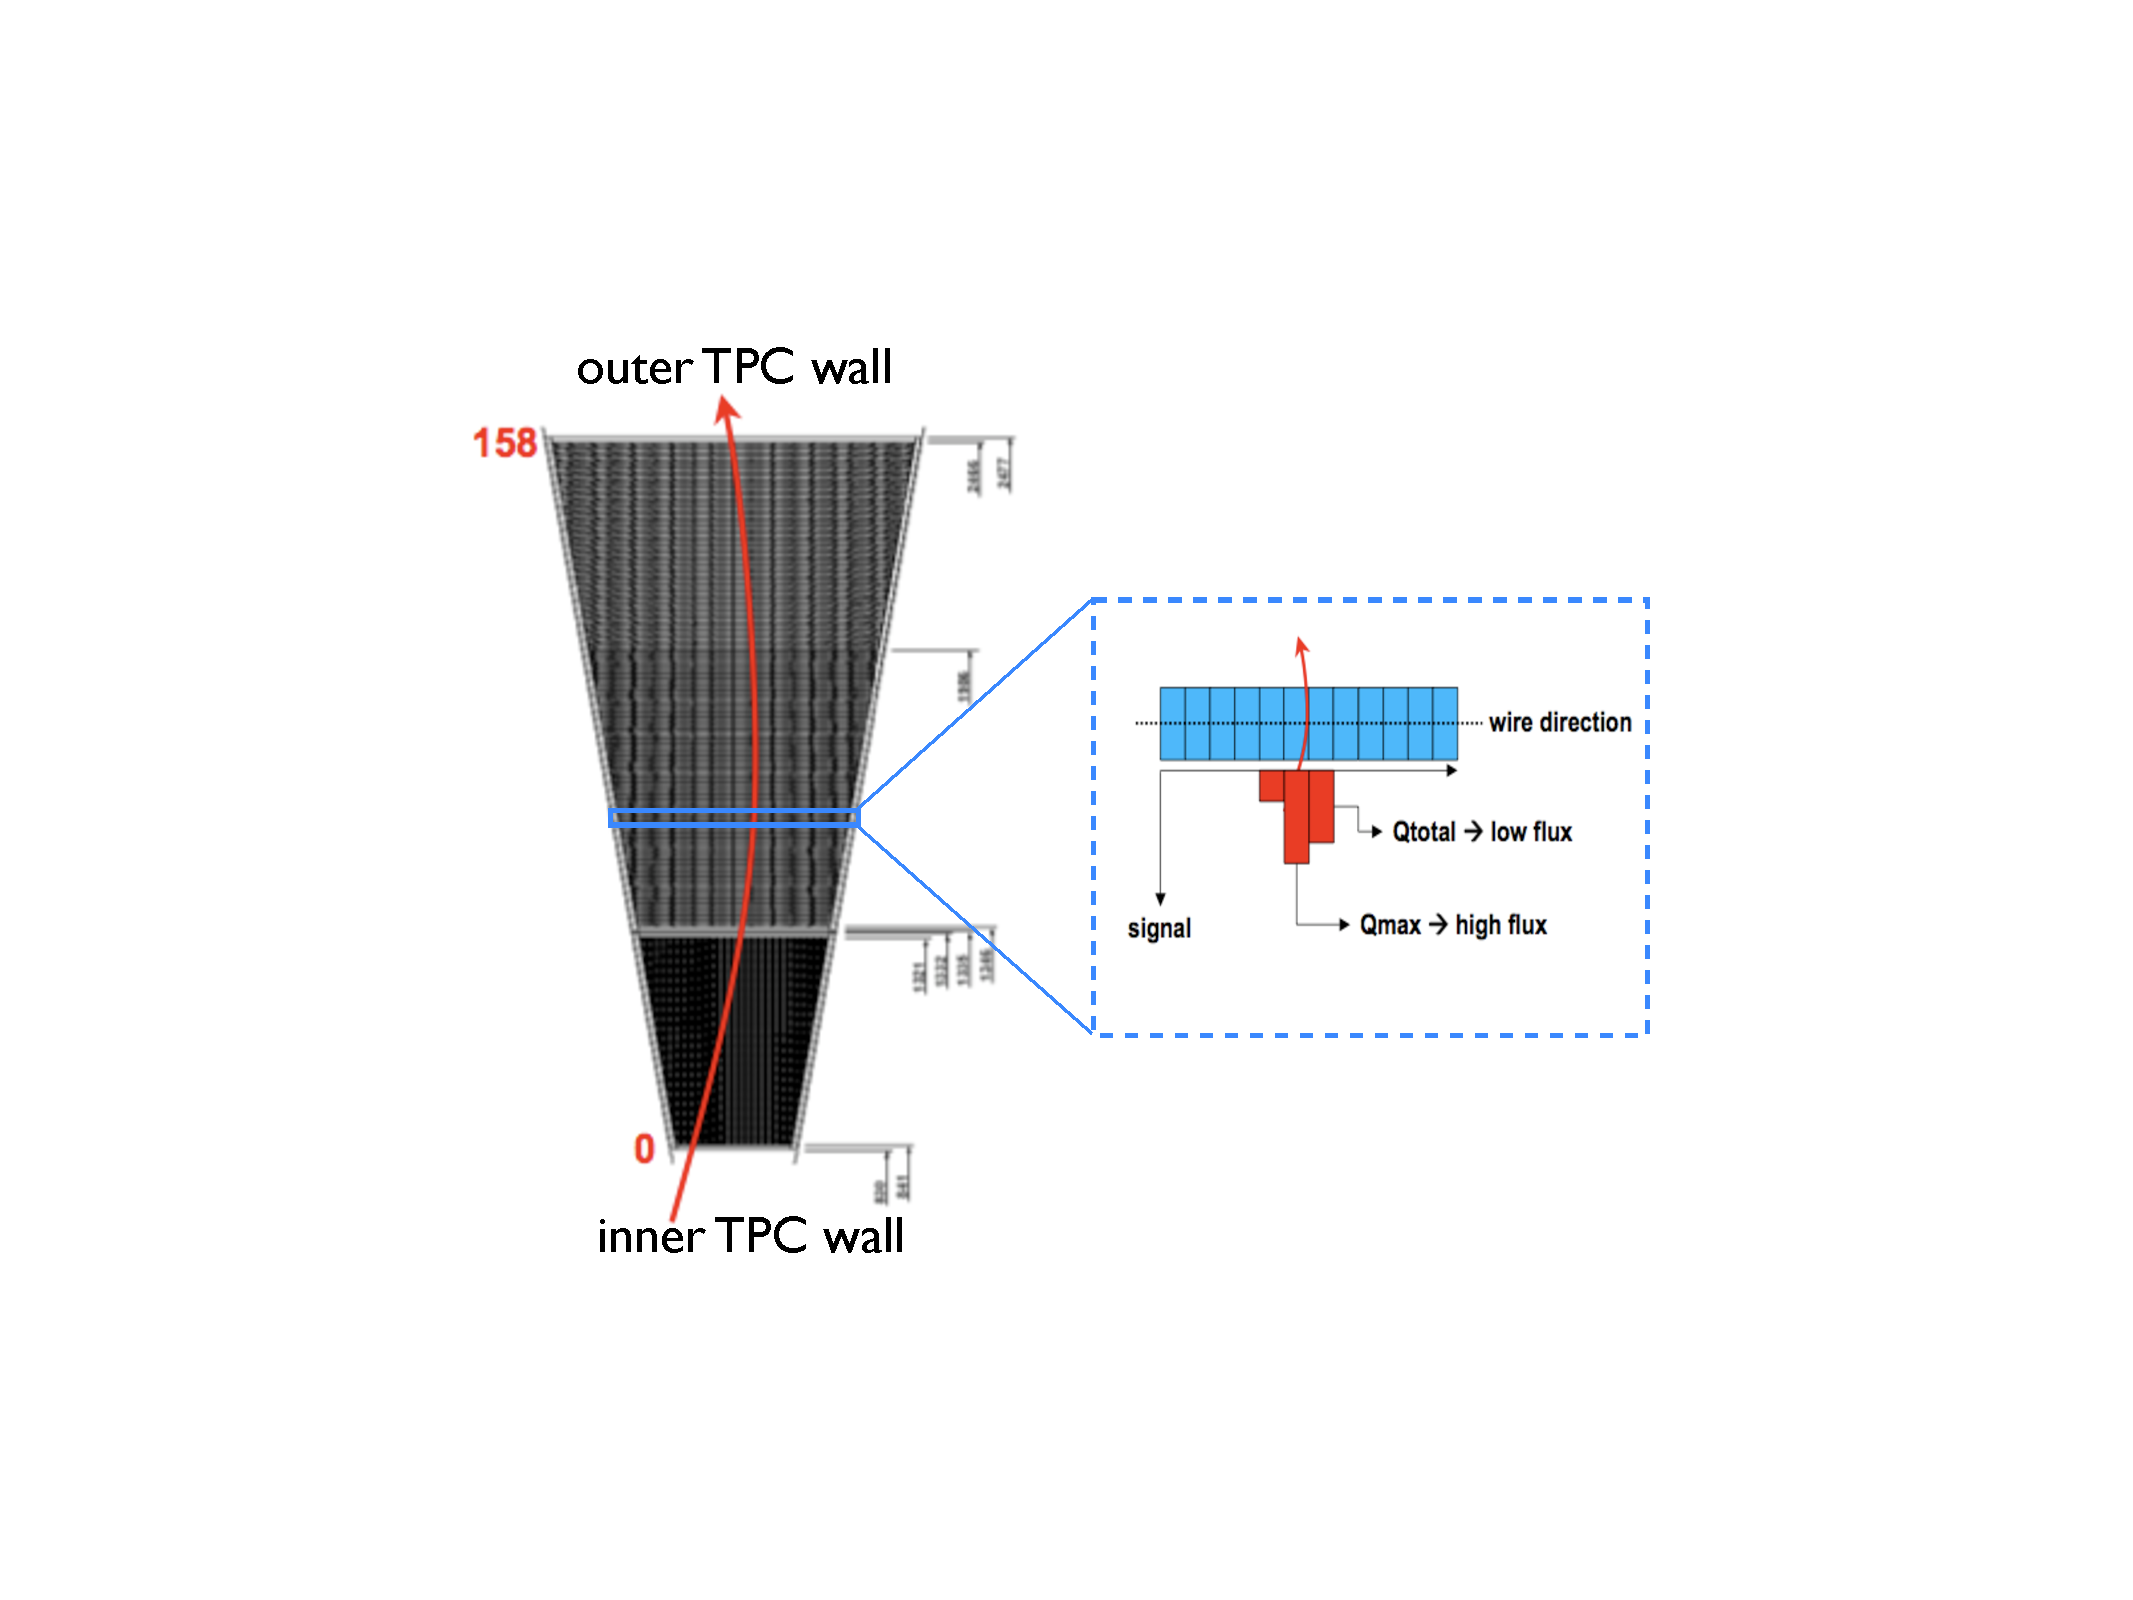
\includegraphics[width=0.6\textwidth]{figures/TPCpadRows}
\caption{A charged particle in one TPC sector. In this case, the track crosses all 159 pad rows (63 in the inner read-out chamber and 96 in the outer read-out chamber).}
\label{figTPCpadRows}
\end{center}
\end{figure}

	
	\item[Findable clusters.] The number of findable clusters is the number of geometrically possible clusters which can be assigned to a track. It takes into account dead zones due to chamber boundaries or the limited $\eta$-acceptance. For the time being, clusters on dead front-end cards are counted as findable.

\medskip	
	{\it Number of findable TPC clusters:} $n_{find}$ / {\tt AliESDtrack::GetTPCNclsF() }
\medskip
	
	\item[Non-findable clusters.] If a track crosses the boundary between two chambers or leaves the $\eta$-acceptance, the clusters in this area are declared as non-finable.
	
	\item[Missing cluster / cluster below threshold.] Findable clusters can be missing, because their charge is below threshold (e.g. due to baseline shifts etc.). They can be identified by looking into the neighboring pad-rows, e.g. if there is no reconstructed cluster on pad row $i$, but clusters are found on the pad rows $i-1$ and $i+1$ (or $i-r$ and $i+r$ in general). The number of clusters below threshold is called $n_{miss}$.
		
        \item[Number of crossed rows $n_{eff}$.] The relevant quantity for the $p_{t}$-resolution of a track is the effectively sampled track length of a particle in the TPC, because the resolution scales roughly $\propto \frac{1}{\sqrt{n_{cl}}}$ (statistics) and  $\propto \frac{1}{n_{eff}^{2}}$ (lever arm) where $n_{eff} = n_{cl} + n_{miss}$. The number is available via the {\it AliRoot}-Function:
	
\medskip
	{\it Number of crossed rows:} $n_{eff}$ / {\tt AliESDtrack::GetTPCClusterInfo(r = 2,1)}.
\medskip

	In this particular case ($r = 2$), a missing cluster is assigned if a cluster is found on one of the two neighboring pad-rows. The number of crossed rows $n_{eff}$ can also be called effective cluster track length. We can consider the following example: Imagine a charged particle enters the TPC at the inner wall with a $p_{t}$ in such a way that it would cross all pad crows in an active area, but it undergoes a catastrophic hadronic interaction in the middle of the TPC, then $n_{find} = 159$, but $n_{eff} = 80$ and (if e.g. 3\% of the clusters were below threshold) $n_{cl} = 76$.
	
	\item[Number of clusters after first iteration.] If a track is recognized as a kink candidate, it is split into a mother and a daughter track. However, the number of assigned clusters $n_{cl}$ is the sum of the clusters assigned to the mother and the daughter. The number of clusters assigned to the mother track are still available via the number of clusters assigned during the first (inward) tracking iteration.
	
\medskip
	{\it Number of clusters after first iteration:} $n_{cl,iter1}$ / {\tt AliESDtrack::GetTPCNclsIter1()}.
\medskip

		
	\end{description}

\subsection{Track parameters}

There are two types of relevant track parameters for a TPC based data analysis: {\it global} (track parameters are updated with inner detectors, i.e. the ITS) and {\it TPC stand-alone (TPC-SA)}.

	\begin{description}
	
	\item[TPC-SA track parameters at the primary vertex.] They describe the track properties at the primary vertex as obtained with the TPC stand-alone. These track parameters are last updated at the inner wall of the TPC and then propagated through the material of the inner detectors to the vertex.

\medskip
		{\tt AliESDtrack::GetTPCInnerParam()}.
\medskip
	

	\item[Global track parameters at the inner TPC wall.] They describe the track properties at the inner wall of the TPC as obtained with the global tracking. These track parameters must be used for the particles identification, because the energy loss of a track inside the TPC is a function of the total momentum $p_{tot,TPC}$ inside the TPC. The global track parameters at the inner TPC wall are a good - though not perfect - approximation for this, because the energy loss inside the TPC fill gas is rather small. \footnote{N.B.: The TPC-SA track parameters at the primary vertex should never be used for pid!}
	
\medskip
		{\tt AliESDtrack::GetInnerParam()}.
\medskip

	
	\item[Global track parameters at the primary vertex.] These are the standard parameters of the ESD track and used in the majority of the physics analyses.
	
		
	\item[Global track parameters at the outer TPC wall.] They are only stored in the AliESDfriends and are usually not relevant for physics analysis.
		
	\end{description}

\subsection{PID related quantities}

\begin{description}

	\item[Energy loss $dE/dx$.] A charged particle traversing the TPC fill gas is losing energy mainly via ionization processes. The mean energy loss $dE/dx$ per unit path length can be described with the Bethe-Bloch formula
	
\begin{equation}
 \langle{dE\over dx}\rangle = {4\pi N e^{4} \over mc^{2}} {Z^{2} \over \beta^{2}} \Bigl(\ln{2mc^{2}\beta^{2}\gamma^{2} \over I} - \beta^{2} - {\delta(\beta) \over 2} \Bigr) \; .
 \label{eq.:Bethe}
\end{equation}

	\item[Energy deposit.] If the energy transfer to the ionized electron exceeds a certain value, the range of the ionized electron becomes so large, that it escapes from the sampling of the charge signal of a given track. In addition to this, some of the energy loss also results only in excitation of the fill gas atoms and no electrons are released. The detectable deposited energy of a track in a given pad-row is therefore slightly different from the energy loss of the charged particle.
	
	\item[Maximum cluster charge $Q_{max}$.] The maximum cluster charge represents the maximum value of all digits in a cluster as shown in figure \ref{figTPCpadRows}.
	
	\item[Total cluster charge $Q_{tot}$.] The total cluster charge is given by the sum of all digits in a cluster. It corresponds to the energy deposit of a track on a given pad-row.
	
	\item[TPC dE/dx signal $S$.] Because of the long tail towards higher energy losses in the distribution function of the cluster charge, the average energy deposit is not a good estimator as it would be for a Gaussian distribution. Therefore, the so-called truncated mean is used. The truncated mean $S$ of all cluster charges, also called the {\it TPC $dE/dx$ signal}, is defined as the average over lowest values, which correspond to a 60\%-fraction of the whole sample.  The values of $S$ follow an almost perfect Gaussian distribution.

\medskip
		{\it TPC dE/dx signal $S$} / {\tt AliESDtrack::GetTPCSignal()}.
\medskip
	
	\item[Number of clusters used for PID $n_{pid}$.] Clusters which are located very close to the chamber boundaries or from overlapping tracks are not used for the calculation of the TPC dE/dx signal. Therefore the number of clusters used for the calculation of the dE/dx-signal can be different from the number of clusters of a track. This quantity is of important relevance for the dE/dx-resolution.
	
	{\it Number of clusters used for pid:} $n_{pid}$ / {\tt AliESDtrack::GetTPCsignalN()}.
	
\end{description}

\section{Recommendation for TPC Cluster Selection}

One of the major systematic error in the physics analysis is introduced by selection criteria on the number of clusters. Based  on experience with TPC data of 2009 and 2010, it is known that TPC gain and baseline variation influence the distribution of found clusters up to  30\% level. This variation is time, energy loss, and running condition dependent and it is only partially described in the MC. However, this variation influences the TPC tracking performance only to the level of $\sqrt{1 - n_{miss}/n_{find}}$.


Most analyses cut on the number of found TPC Clusters divided by the number of findable clusters $\varepsilon_{thr} = \frac{found clusters}{findable clusters}$. However the number of found clusters is not robust as explained below.
Instead the TPC group has introduced a new variable - the ratio of number of crossed rows to the number of findable clusters - which is almost independent on track multiplicity and $\eta$. At the end of this section a recommendation on what variables to cut on in order to achieve good $p_{t}$ resolution and fake removal is given. \newline

\noindent TPC clusters can be lost due to unknown reasons or because their charge is below threshold (caused by the front-end electronics; these clusters are called missing clusters). The threshold of the cluster finder approaches the digital threshold (due to the 1pad cluster functionality). The unknown reasons summarize effects such as dead zones, missing partitions and decays.
$\varepsilon_{thr}$ depends on the digital threshold, on multiplicity, energy loss, drift length and track angle. The later three determine simply the amplitude of the signal. \newline
\noindent The dependence of $\varepsilon_{thr}$ on these is shown in figures \ref{fig_2dim_dep_a} and \ref{fig_2dim_dep_b} for PbPb data taken in 2010.
 The different colors correspond to different energy loss. The lowest lying distribution corresponds to low energy loss the one overlaying all high energy loss. Multiplicity is defined by the number of contributors to the TPC vertex.
For better visualization the plots \ref{fig_2dim_dep_a} and \ref{fig_2dim_dep_b} are projected in slices of multiplicity and $\eta$. Then for a given threshold, a limit removing the lower x\% of the distribution, the related $\varepsilon_{thr}$ is determined. The output is shown in Figures \ref{fig_1dim_dep_a} and \ref{fig_1dim_dep_b}. A clear dependence on track multiplicity and $\eta$ is seeable.

\noindent In Figures \ref{fig_2dim_dep_c} and \ref{fig_2dim_dep_d} as well as \ref{fig_1dim_dep_c} and \ref{fig_1dim_dep_d} one can see the corresponding plots for the ratio of number of crossed rows to the number of findable clusters. The ratio, the newly introduced variable, is almost independent from energy loss, multiplicity and $\eta$ (z-direction). The dip in the $\eta$-plot is due to the crossing of tracks with the central cathode.



\begin{figure}[htbp]
\centering \mbox{
  \subfigure[$\varepsilon_{thr}$ vs $\eta$]{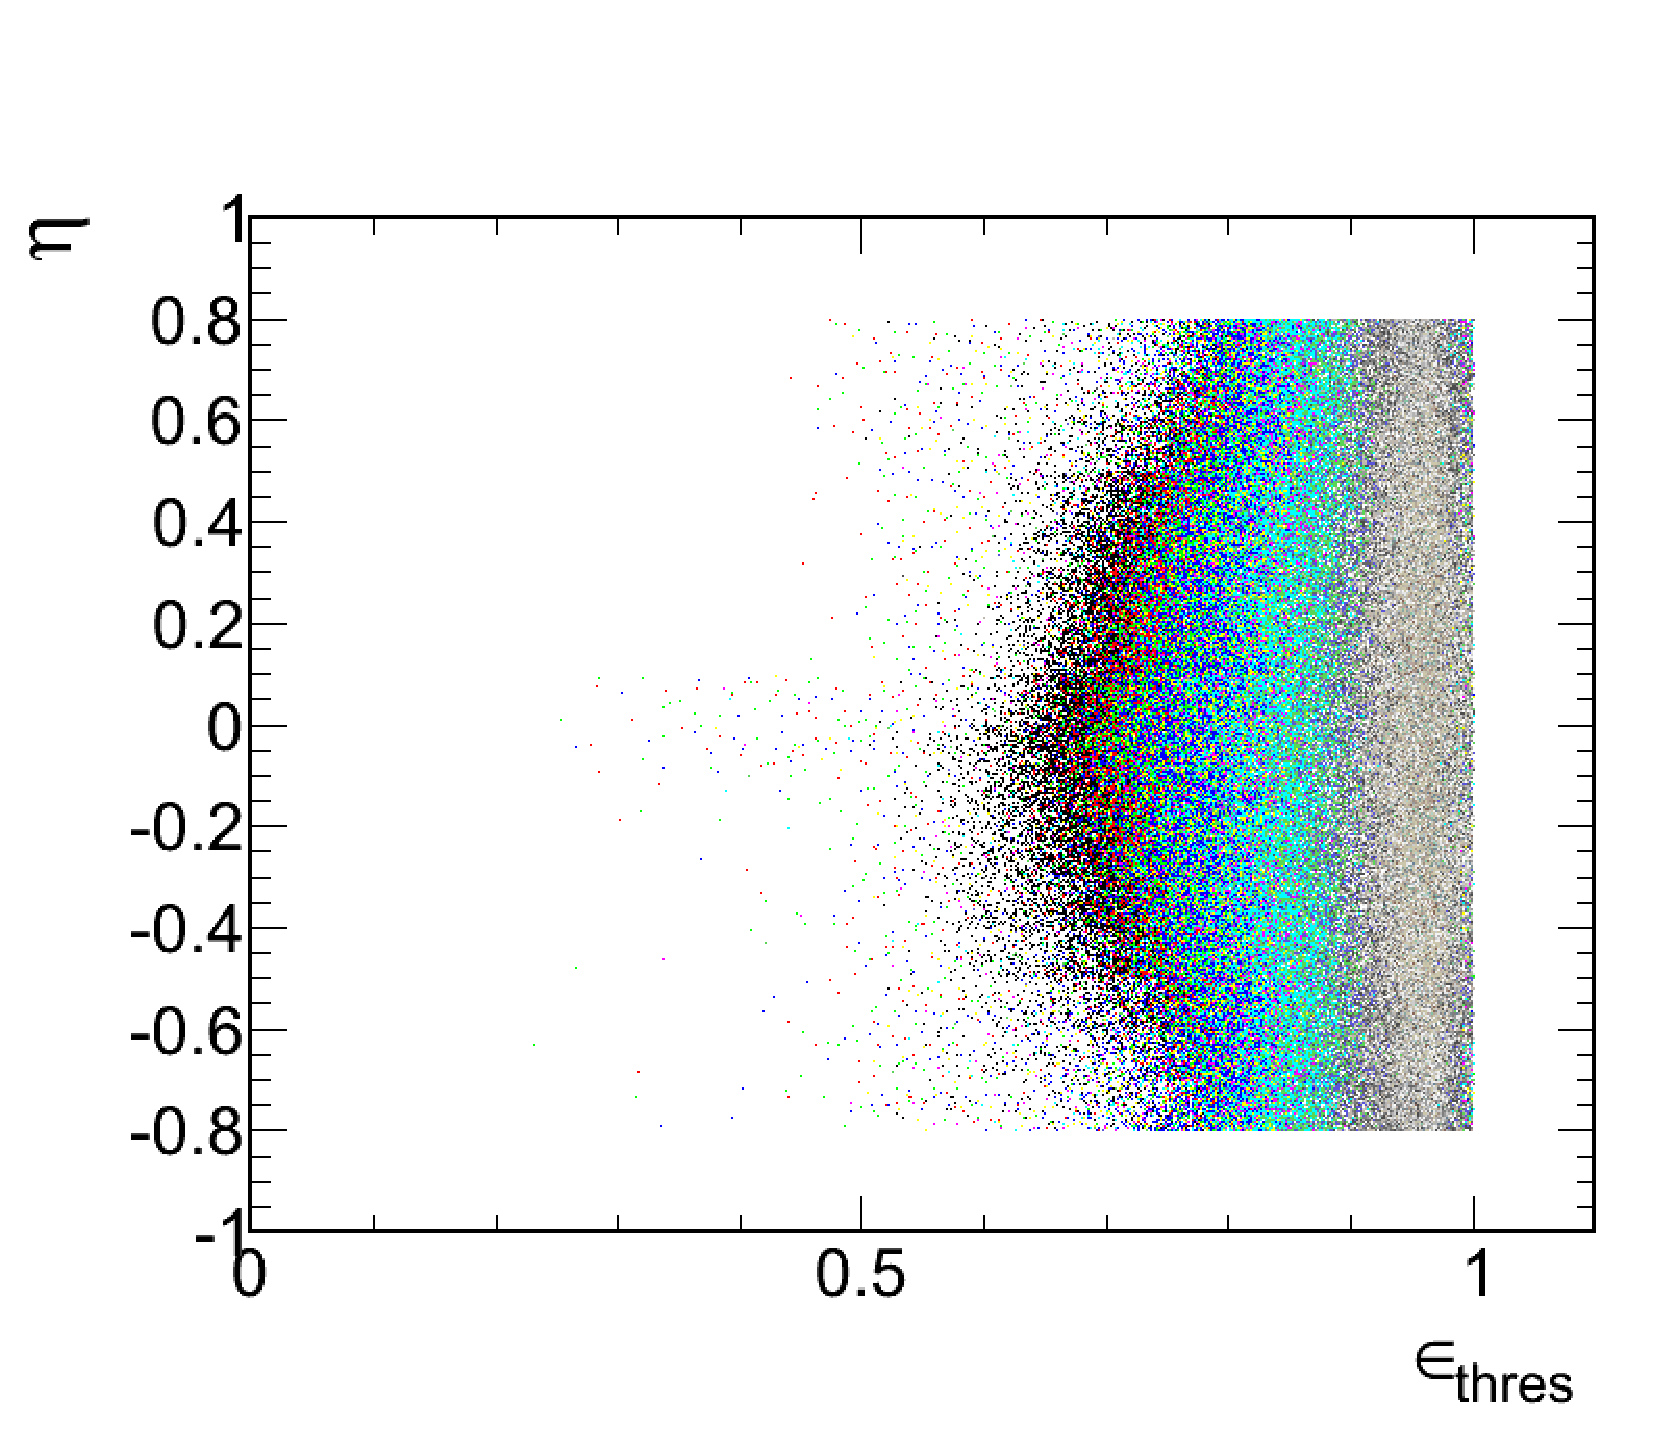
\includegraphics[width=0.6\mylinewidth]{figures/new_ethres_vs_eta.pdf}\label{fig_2dim_dep_a}}
  \subfigure[$\varepsilon_{thr}$ vs multiplicity]{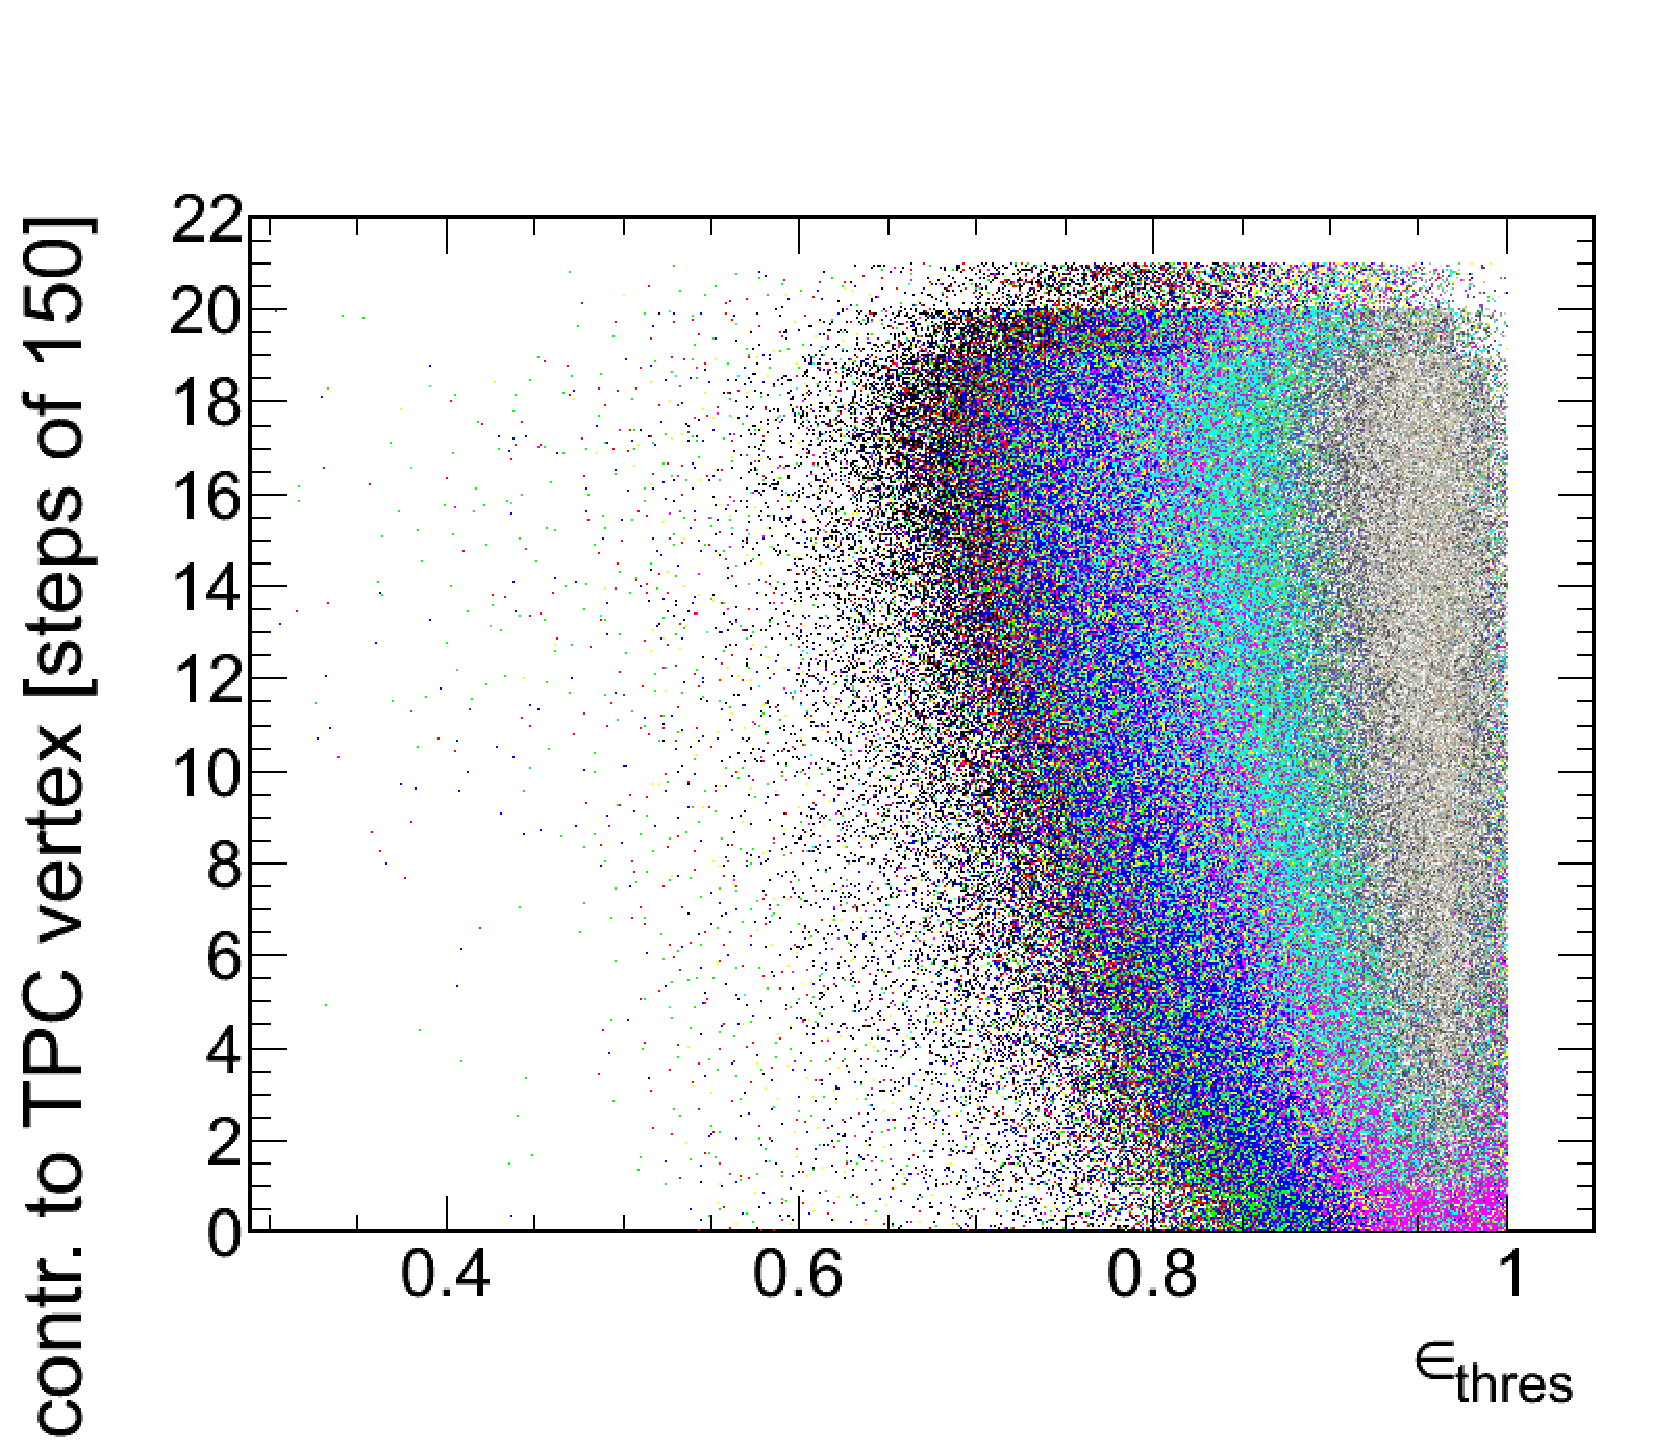
\includegraphics[width=0.6\mylinewidth]{figures/new_ethres_vs_multi.pdf}\label{fig_2dim_dep_b}}}
\centering \mbox{
  \subfigure[Number of crosses rows divided by number of findable clusters vs $\eta$]{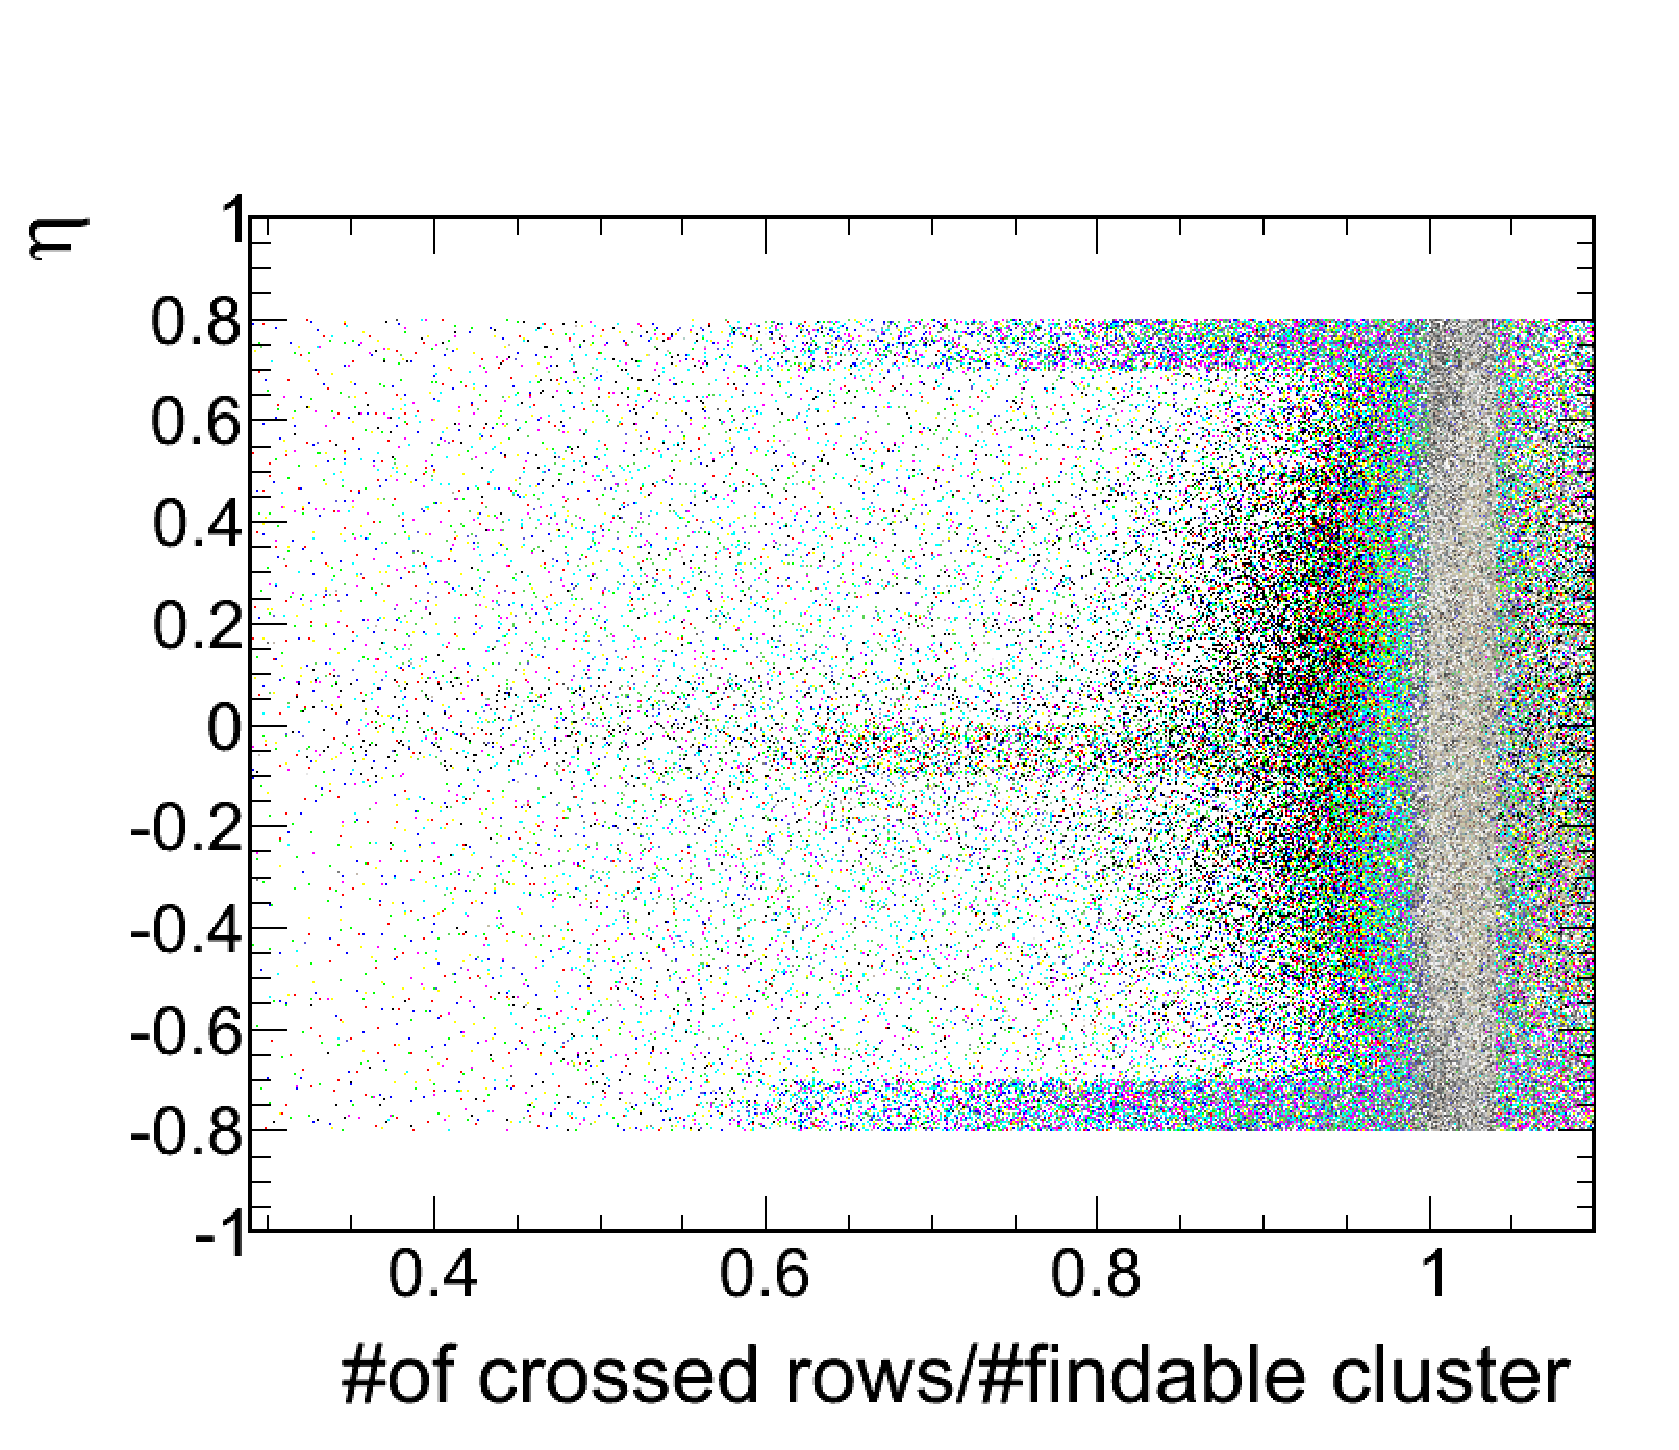
\includegraphics[width=0.6\mylinewidth]{figures/new_cros_vs_eta.pdf}\label{fig_2dim_dep_c}}
  \subfigure[Number of crosses rows divided by number of findable clusters vs multiplicity]{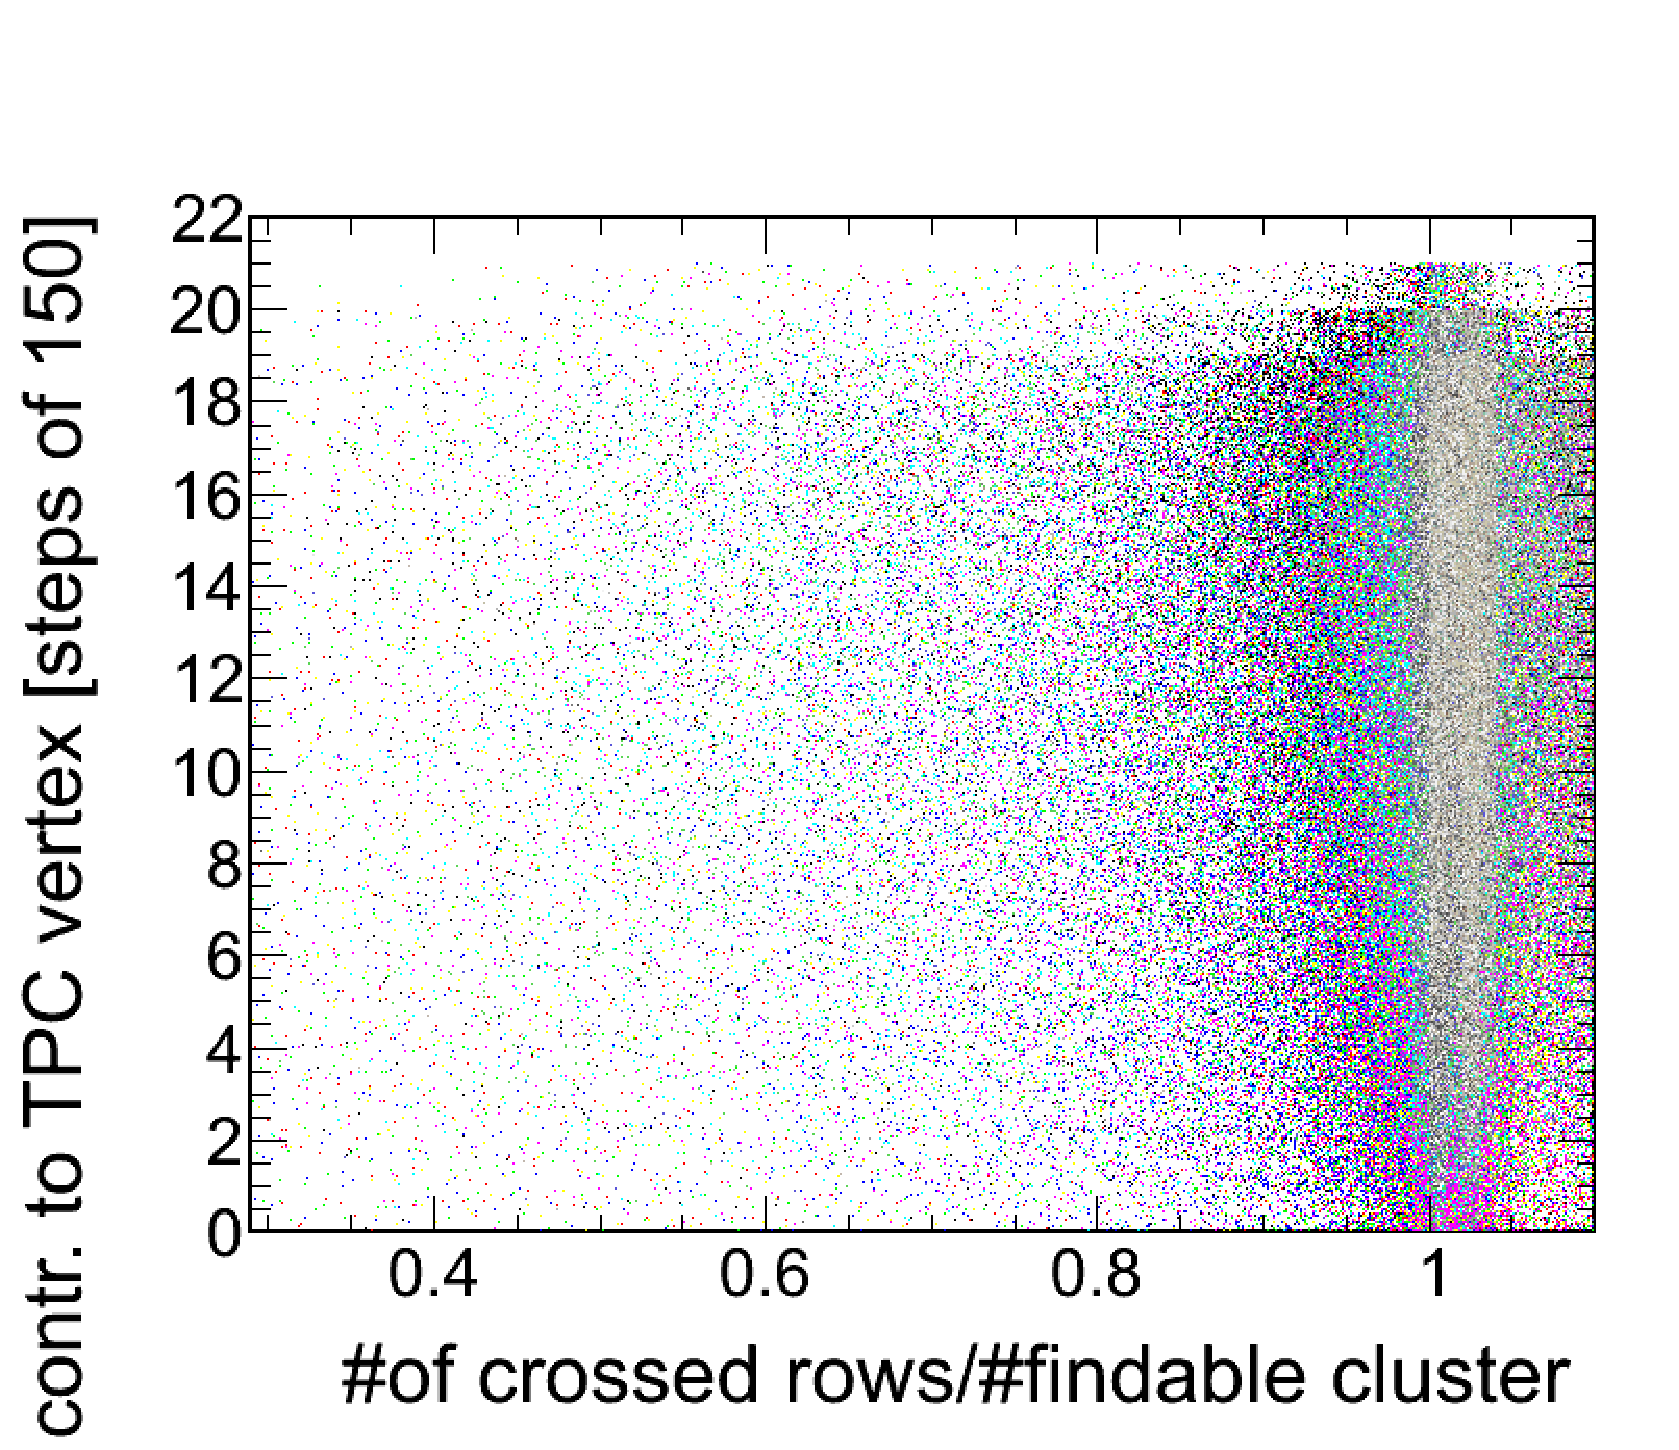
\includegraphics[width=0.6\mylinewidth]{figures/new_cros_vs_multi.pdf}\label{fig_2dim_dep_d}}}
  \caption[]{$\varepsilon_{thr}$ and number of crosses rows divided by number of findable clusters vs $\eta$ and multiplicity for PbPb data taken in 2010. Multiplicity is defined by the number of contributors to the TPC vertex. The different colors correspond to different energy loss. The lowest lying distribution corresponds to low energy loss the one overlaying all high energy loss.}
\label{fig_2dim_dep}
\end{figure}

\begin{figure}[htbp]
\centering \mbox{
  \subfigure[$\varepsilon_{thr}$ vs $\eta$ for various thresholds]{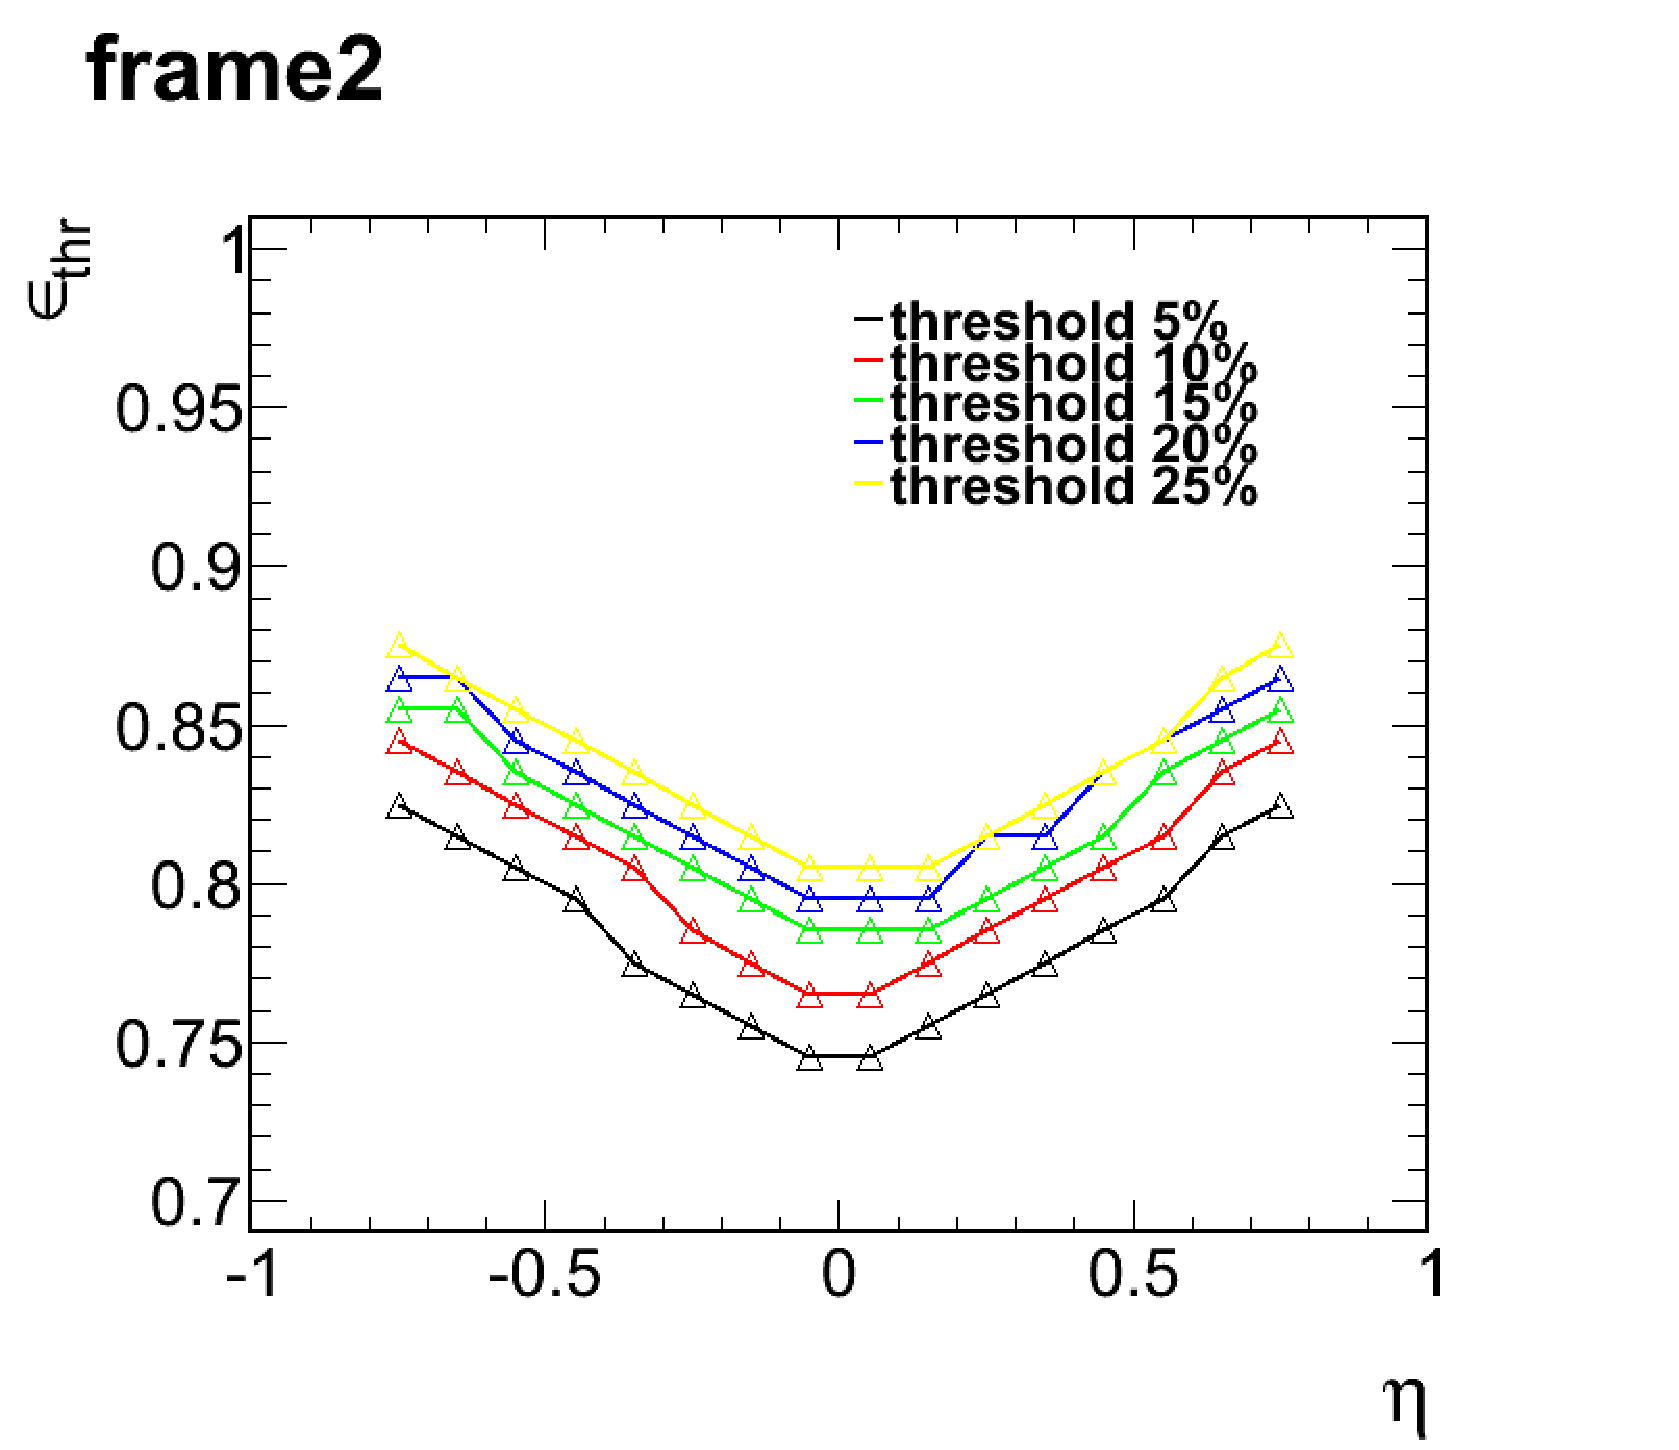
\includegraphics[width=0.6\mylinewidth]{figures/ethres_vs_eta_threshold.pdf}\label{fig_1dim_dep_a}}
  \subfigure[$\varepsilon_{thr}$ vs multiplicity for various thresholds]{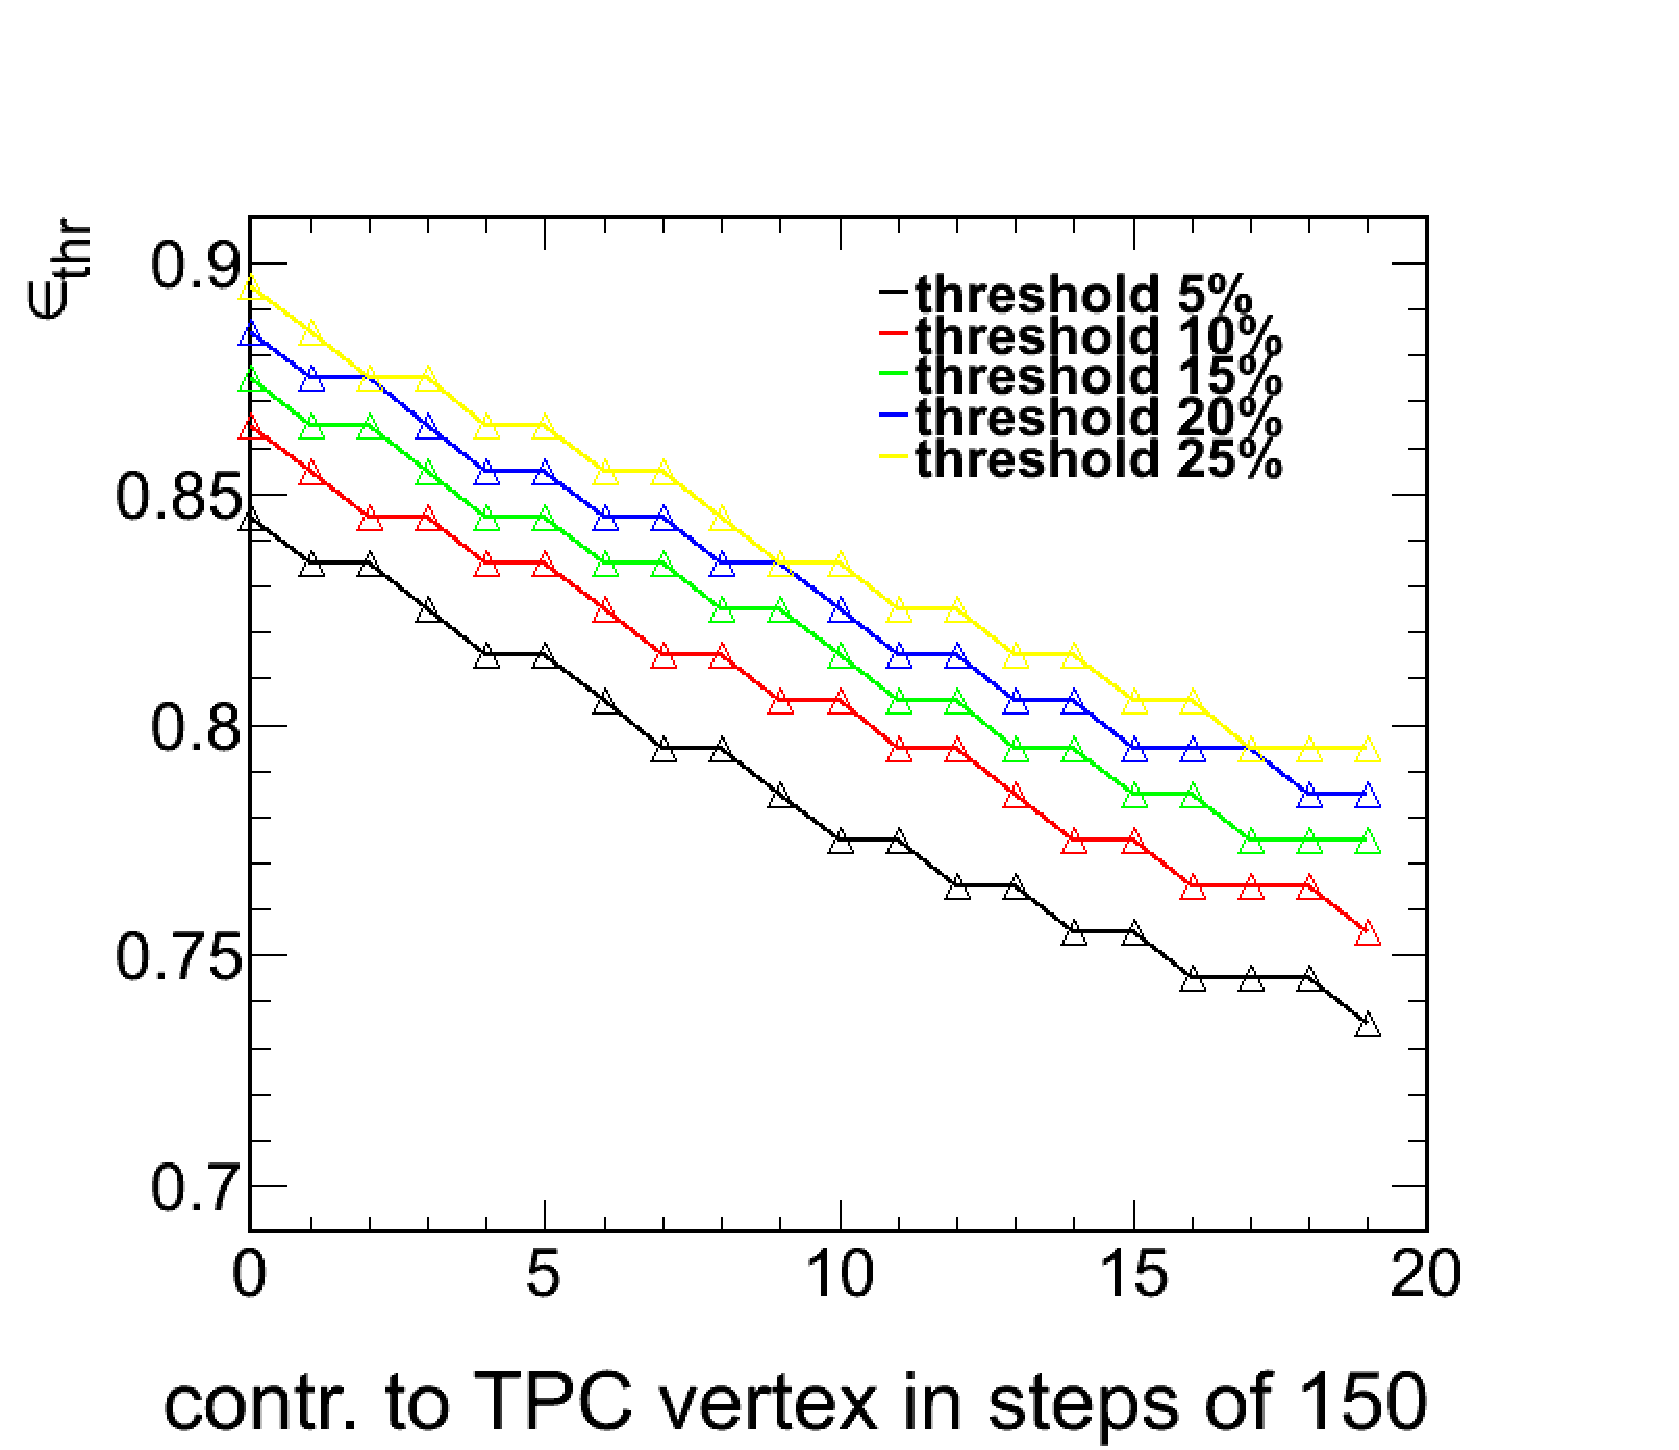
\includegraphics[width=0.6\mylinewidth]{figures/ethres_vs_multi_thresholds.pdf}\label{fig_1dim_dep_b}}}
\centering \mbox{
  \subfigure[Number of crosses rows divided by number of findable clusters vs $\eta$ for various thresholds]{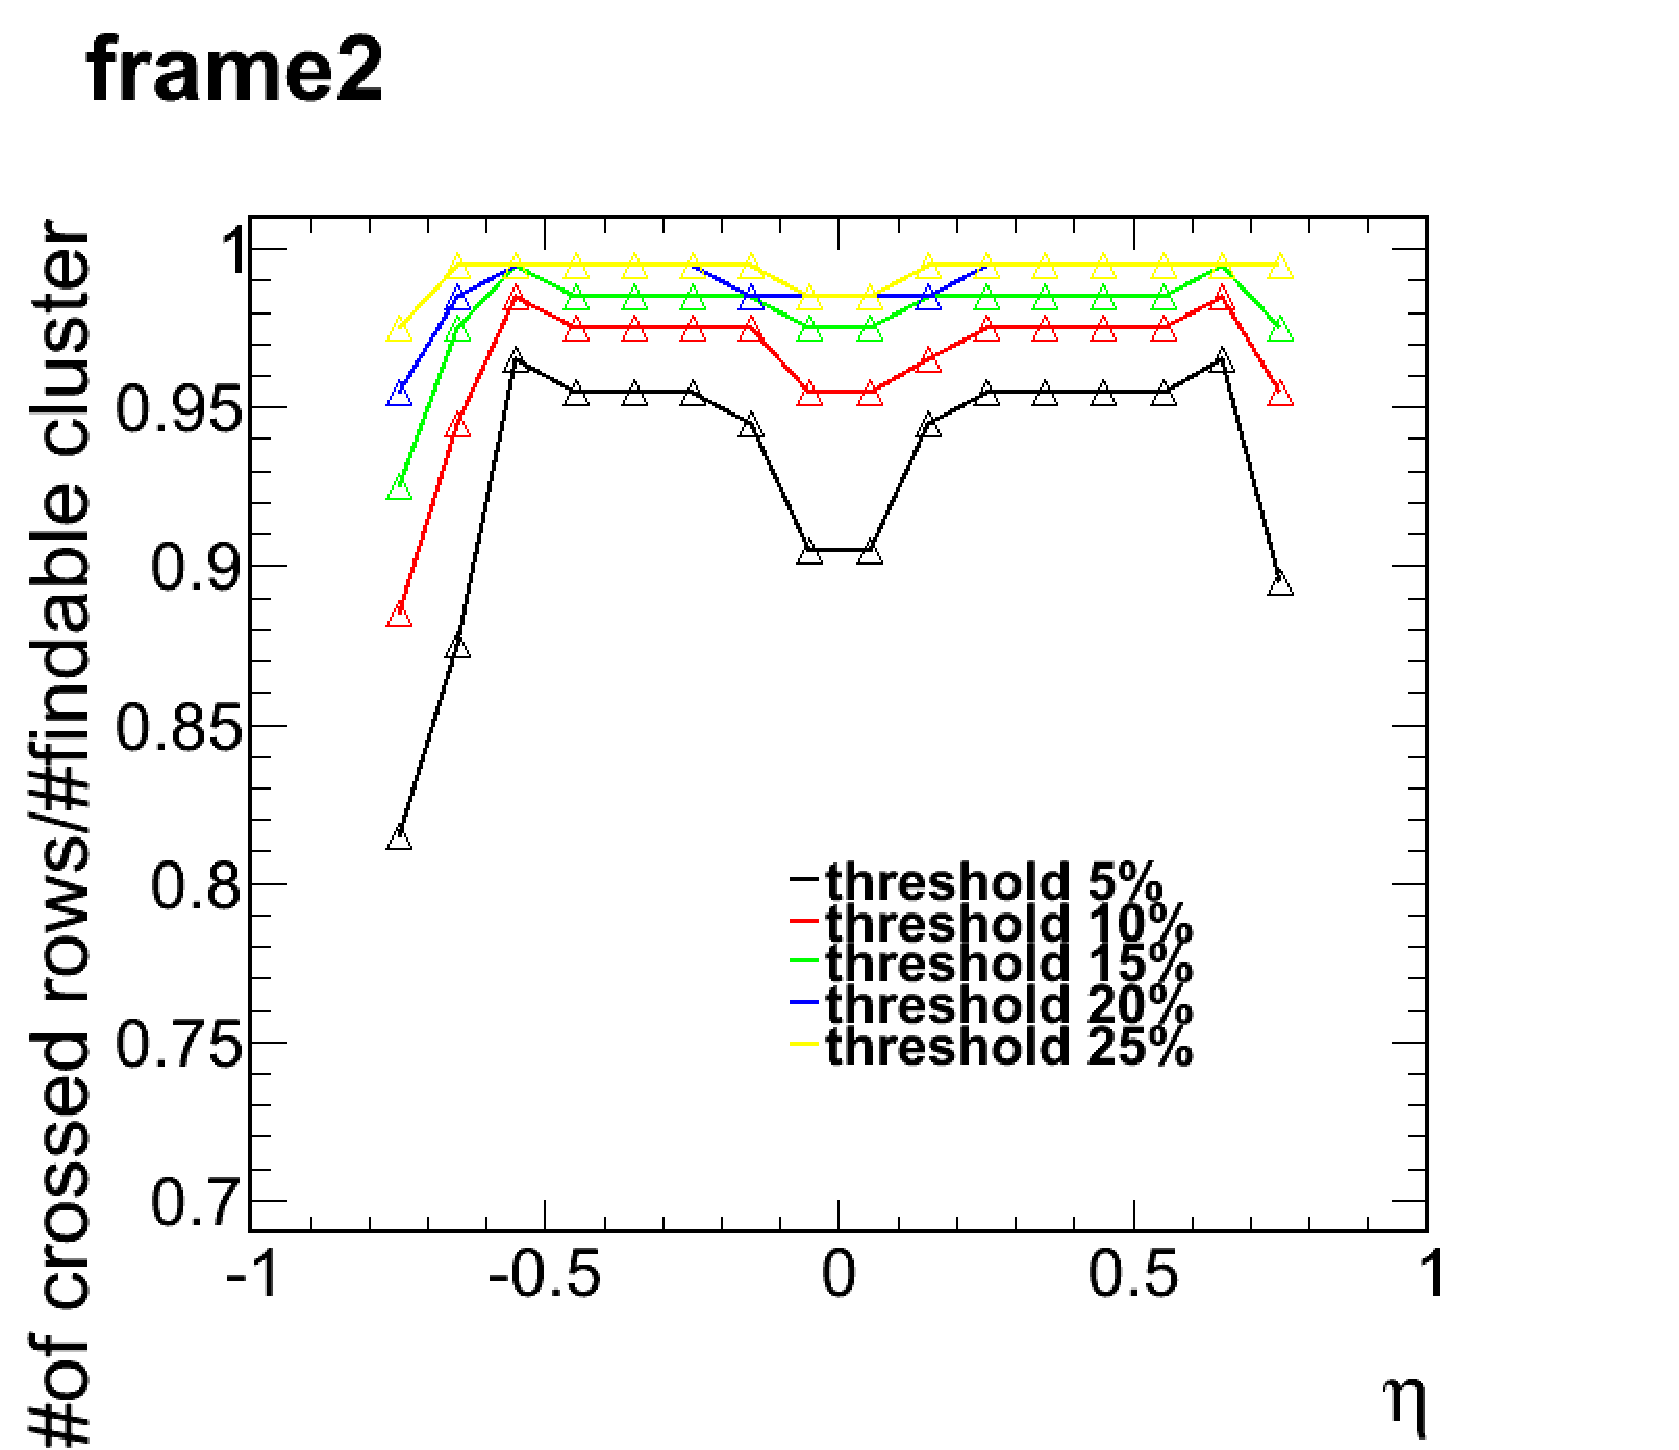
\includegraphics[width=0.6\mylinewidth]{figures/ncrossed_vs_eta_thres.pdf}\label{fig_1dim_dep_c}}
  \subfigure[Number of crosses rows divided by number of findable clusters vs multiplicity for various thresholds]{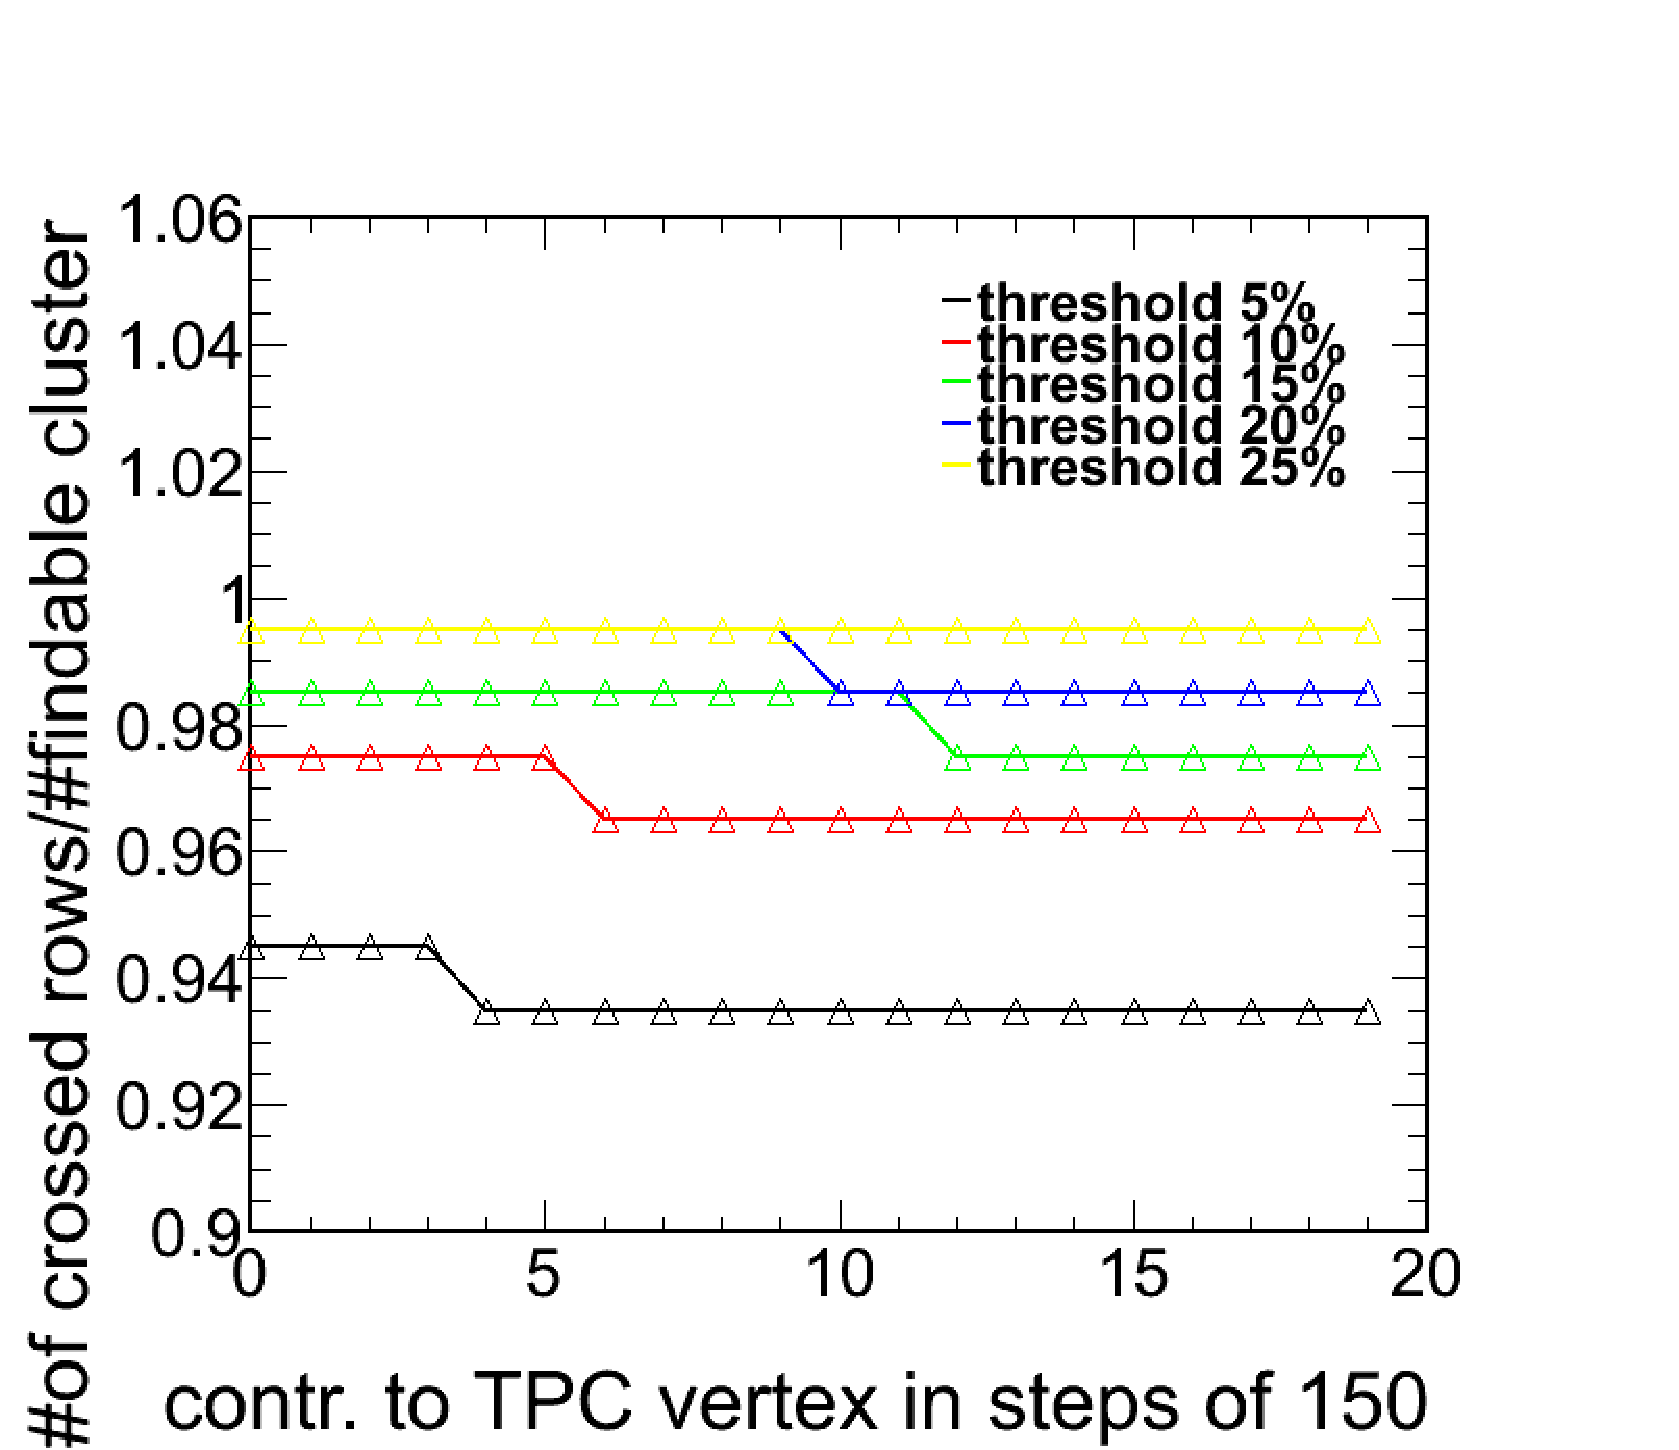
\includegraphics[width=0.6\mylinewidth]{figures/crossedrows_vs_multi_thres.pdf}\label{fig_1dim_dep_d}}}
  \caption[]{$\varepsilon_{thr}$ and number of crosses rows divided by number of findable clusters for a given threshold as a function of $\eta$ and multiplicity for PbPb data taken in 2010. Multiplicity is defined by the number of contributors to the TPC vertex.}
\label{fig_1dim_dep}
\end{figure}

\subsection{Available Variables and Cut Recipes} \label{subsection_qavariables}
Analyses with the TPC can make use of the following QA variables:
\begin{enumerate}
\item Number of TPC clusters
\item Number of findable clusters
\item Number of crossed rows
\item Number of clusters in crossed rows
\item Covariance matrix elements
\item All combinations and ratios of the items above
\end{enumerate}

\noindent To achieve good $p_{t}$ resolution for high momenta a cut on the number of crossed rows and the covariance matrix elements are recommended. Cuts on ITS remove already a lot of fakes. Further improvement is reached with  a minimal cut on the number of crossed rows and on the ratio of number of crossed rows to number of findable clusters. The application of the cuts depends on the type of analysis, e.g. the cuts proposed for further fake removal do not apply for V0 analysis (gamma conversion, kinks, etc.).
For other types of analyses we recommend to accept only tracks with a ratio of number of crossed rows to number of findable clusters of larger than 0.83. This has the advantage of also being independent of one missing partition in the read out (see Fig. \ref{fig_pp_mc_data}). \newline 
\noindent Figure \ref{fig_pp_mc_data} shows the ratio of number of crossed rows to findable clusters for experimental data (pp LHC10d) and for the respective MC sample. The distribution for experimental data has a small peak at slightly below 0.9 and then increases in comparison to the MC distribution slower. This is due to a missing partition. Depending on the angle with which the track passes the missing partition up to all clusters are correspondingly not recorded. \newline
\noindent Though given the anchor runs MC will not follow the time dependence due to missing partitions in data. Further discrepancies between MC and data are due to different species abundance. Thus a comparison of data to MC is only possible by keeping the upper x\% of the distributions in both MC and data.

A summary of the recommended cuts can be found in Table \ref{table_cuts} \newline \newline \newline

\begin{figure}[htbp]
\begin{center}
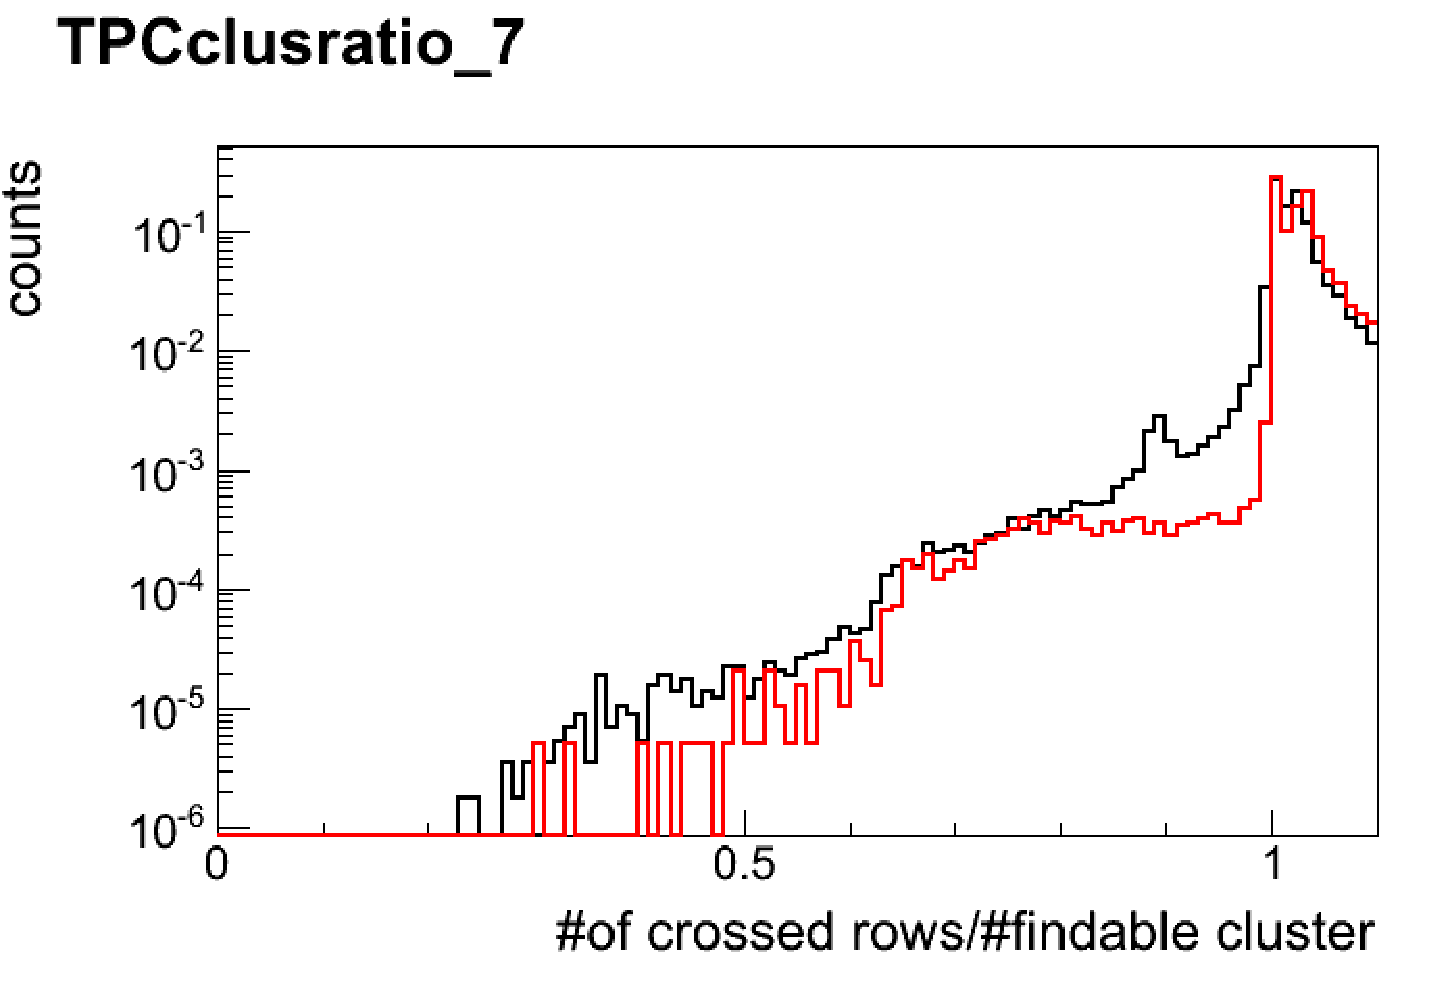
\includegraphics[width=0.6\textwidth]{figures/pp_mc_data.pdf}
\caption{Number of crosses rows divided by number of findable clusters for pp data LHC10d (black) and the corrresponding MC sample (red). Shown for tracks with an energy loss of 70-79 and an event multiplicity of 30-45 contributors to the TPC vertex.}
\label{fig_pp_mc_data}
\end{center}
\end{figure}

\begin{table}[\htb]
 \begin{center}
\begin{tabular}{l||l}
\hline
\textbf{Goal} & \textbf{Cut} \\
\hline \hline
Good pt resolution  & Cut on 4. + 5. for high momenta \\
Fake removal & Minimal cut on 3. + on 3./2. \\
MC vs real data & Keep upper x\% of distribution in MC and data
respectively \\
\end{tabular} 
\end{center}
\caption[]{Recommended cuts to achieve good $p_{t}$ resolution and fake removal. The numbers are explained at the beginning of Section \ref{subsection_qavariables}.} \label{table_cuts}
\end{table} 

\subsection{QA Selection based on the estimated resolution} \label{subsection_COVARvariables}

The tracking performance of ALICE detector is described by   covariance matrix of tracks. The actual uncertainty of the track parameters depends on many parameters:
\begin{itemize}
\item At high track momenta the resolution is determined mainly by track topology, detectors contributing to the measuremant (TPC only, constrained parameters, Combined tracks) and by quality of alignment and calibration.
\item At low momenta the track uncertainty is determined by multiple scatterring and by energy loss in the material (PID dependent)    
\end{itemize}

Following empirical  parameterization can be used to describe the mean uncertanties of the track parameters:
\begin{equation}
 \sigma_{xx}=k_{xx0}\sqrt{1+k_{xx1}/p_{t}^{k_{xx2}}}\sqrt{dEdx/dEdx_{MIP}}
 \label{eq.:TrackResol}
\end{equation}


\begin{figure}[htbp]
\begin{center}
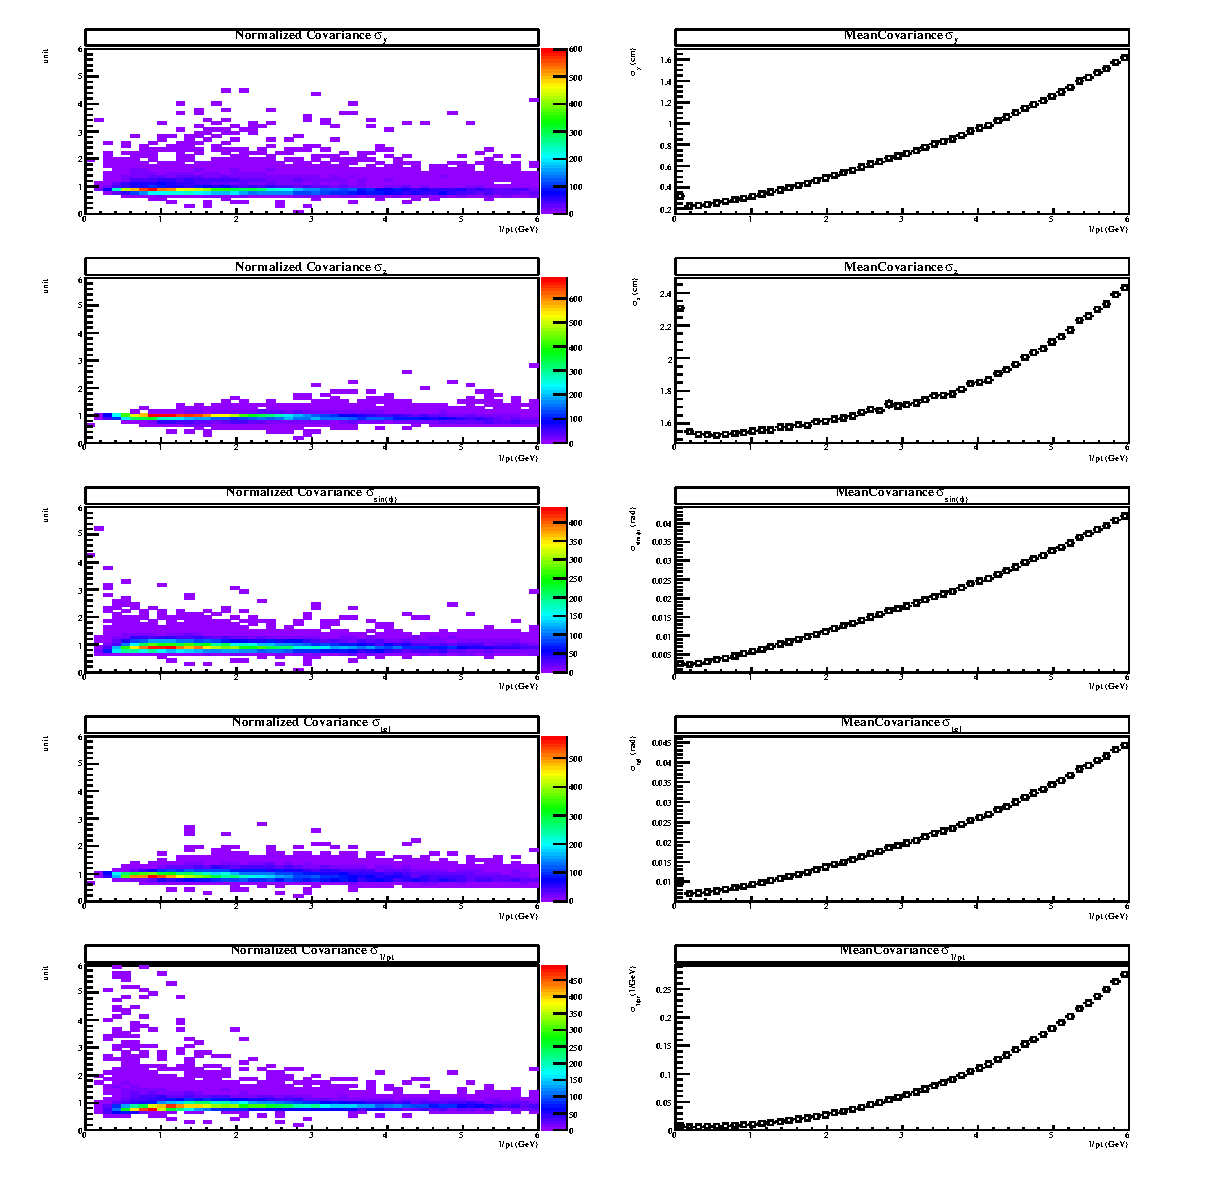
\includegraphics[width=0.8\textwidth]{figures/covarScaledTPC.eps}
\label{fig_CovarTPC}
\end{center}
\caption{Normalized covariance elements and the mean uncerntainty of track parameters for the TPC only tracks at vertex}
\end{figure}

\begin{figure}[htbp]
\begin{center}
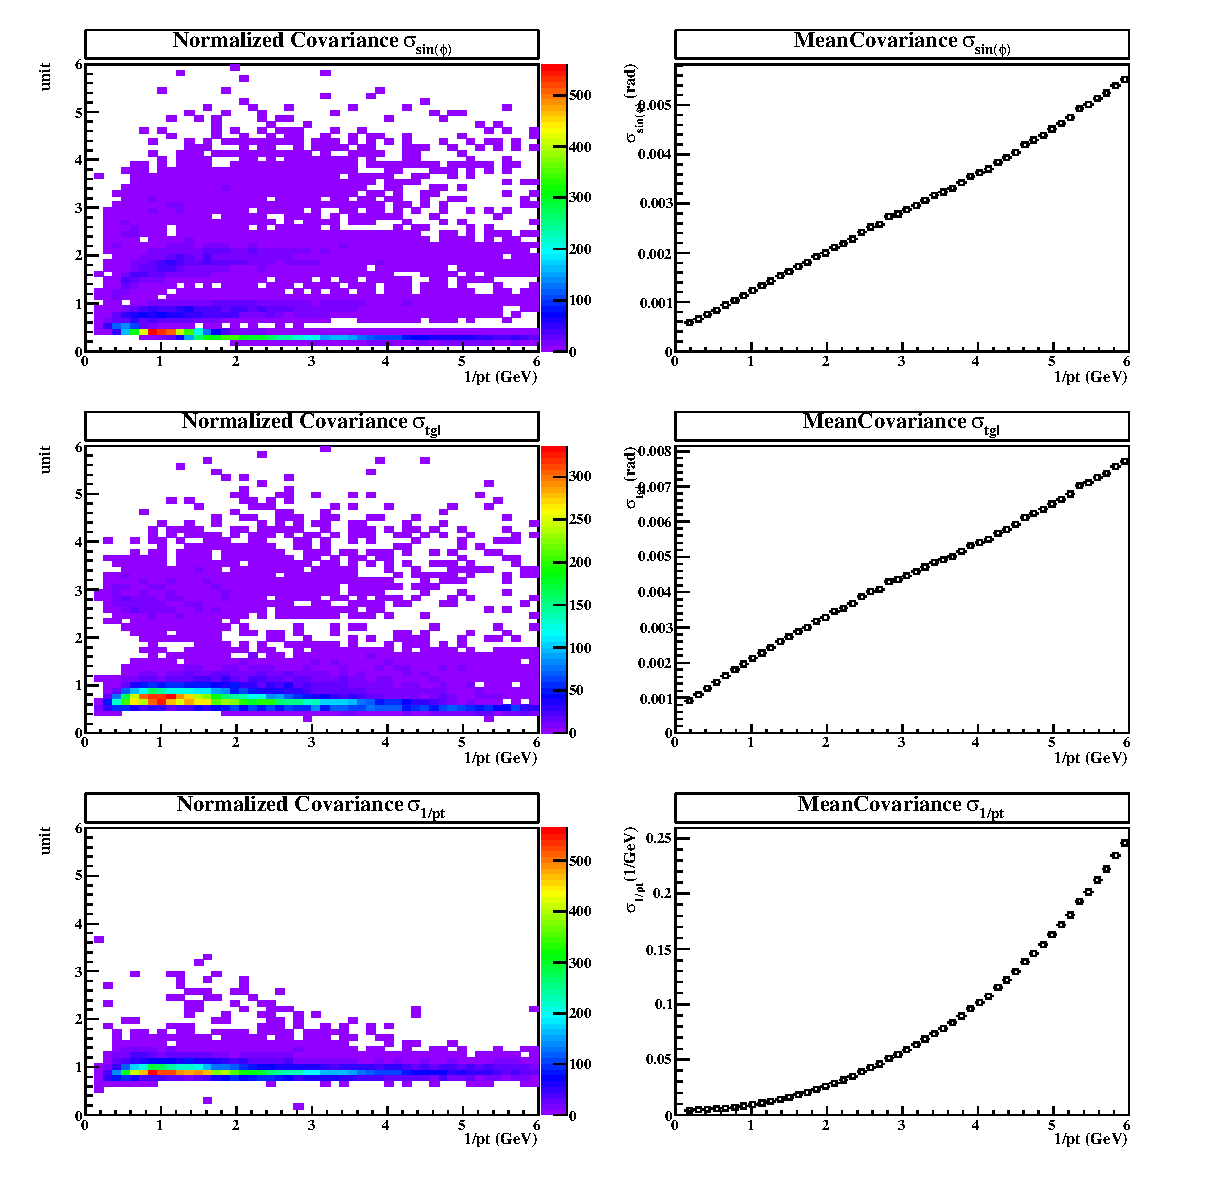
\includegraphics[width=0.8\textwidth]{figures/covarScaledConst.eps}
\label{fig_CovarTPC}
\end{center}
\caption{Normalized covariance elements and the mean uncerntainty of track parameters for the combined constrained  tracks at vertex. Several bands for the uncertainty in the angular measurement due differnt track topology (Presence if the differnt ITS layers).}
\end{figure}




\end{document}
